% add document structure
\documentclass[12pt]{book}
%
%\usepackage{fullpage}
\usepackage{graphicx}
\graphicspath{ {./images/} }
\usepackage{float}
\usepackage{fancyhdr}
\usepackage{amsmath}
\usepackage{amssymb}
\usepackage{booktabs}
\usepackage{xlop}
\usepackage{tikz}

% newcommands
\newcommand{\xdownarrow}[1]{%
  {\left\downarrow\vbox to #1{}\right.\kern-\nulldelimiterspace}
}

% end docmunt sturcture
\begin{document}
\pagestyle{fancy}
\fancyhead{} % clear all header fields
\fancyhead[LE]{\textbf{Programming the 6502}}
\fancyhead[RO]{\textbf{Basic Concepts}}
\fancyfoot{} % clear all footer fields
\fancyfoot[LE,RO]{\textbf\thepage}
\chapter{BASIC CONCEPTS}
\section*{INTRODUCTION}

\indent{This chapter will introduce the basic concepts and definitions relating to computer programming. The reader already familiar with these concepts may want to glance quickly at the contents of this chapter and then move on to Chapter 2. It is suggested, however, that even the experienced reader look at the contents of this introductory chapter. Many significant concepts are presented here including, for example, two's complement, BCD, and other representations. Some of these concepts may be new to the reader; others may improve the knowledge and skills of experienced programmers.}

\section*{WHAT IS PROGRAMMING?}

\indent{Given a problem, one must first devise a solution. This solution, expressed as a step-by-step procedure, is called an algorithm. An algorithm is a step-by-step specification of the solution to a given problem. It must terminate in a finite number of steps. This algorithm may be expressed in any language or symbolism. A simple example of an algorithm is:}
\begin{enumerate}
	\item {insert key in the keyhole}
	\item {turn key one full turn to the left}
	\item {seize doorknob}
	\item {turn doorknob left and push the door}
\end{enumerate}
\indent{At this point, if the algorithm is correct for the type of lock in volved, the door will open. This four-step procedure qualifies as an algorithm for door opening.}

\indent{Once a solution to a problem has been expressed in the form of an algorithm, the algorithm must be executed by the computer. Unfortunately, it is now a well-established fact that computers cannot understand or execute ordinary spoken English (or any other human language). The reason lies in the syntactic ambiguity of all common human languages. Only a well-defined subset of natural language can be "understood" by the computer. This is called a programming language.}

\indent{Converting an algorithm into a sequence of instructions in a pro gramming language is called programming. To be more specific, the actual translation phase of the algorithm into the program ming language is called coding. Programming really refers not just to the coding but also to the overall design of the programs and "data structures" which will implement the algorithm.}

\indent{Effective programming requires not only understanding the possible implementation techniques for standard algorithms, but also the skillful use of all the computer hardware resources, such as internal registers, memory, and peripheral devices, plus a creative use of appropriate data structures. These techniques will be covered in the next chapters.}

\indent{Programming also requires a strict documentation discipline, so that the programs are understandable to others, as well as to the author. Documentation must be both internal and external to the program.}

\indent{Internal program documentation refers to the comments placed in the body of a program, which explain its operation.}

\indent{External documentation refers to the design documents which are separate from the program: written explanations, manuals, and flowcharts.}

\section*{FLOWCHARTING}

\indent{One intermediate step is almost always used between the algorithm and the program. It is called a flowchart. A flowchart is simply a symbolic representation of the algorithm expressed as a sequence of rectangles and diamonds containing the steps of the algorithm. Rectangles are used for commands, or "executable statements." Diamonds are used for tests such as: If information X is true, then take action A, else B. Instead of presenting a formal definition of flowcharts at this point, we will introduce and discuss flowcharts later on in the book when we present programs.}

\indent{Flowcharting is a highly recommended intermediate step be tween the algorithm specification and the actual coding of the solution. Remarkably, it has been observed that perhaps 10\% of the programming population can write a program successfully with out having to flowchart. Unfortunately, it has also been observed that 90\% of the population believes it belongs to this 10\%! The result: 80\% of these programs, on the average, will fail the first time they are run on a computer. (These percentages are naturally not meant to be accurate.) In short, most novice programmers seldom see the necessity of drawing a flowchart. This usually results in "unclean" or erroneous programs. They must then spend a long time testing and correcting their program (this is called the debugging phase). The discipline of flowcharting is therefore highly recommended in all cases. It will require a small amount of additional time prior to the coding, but will usually result in a clear program which executes correctly and quickly. Once flowcharting is well understood, a small percentage of programmers will be able to perform this step mentally without having to do it on paper. Unfortunately, in such cases the programs that they write will usually be hard to understand for anybody else without the documentation provided by flowcharts. As a result, it is universally recommended that flowcharting be used as a strict discipline for any significant program. Many examples will be provided throughout the book.}

\section*{INFORMATION REPRESENTATION}

\indent{All computers manipulate information in the form of numbers or in the form of characters. Let us examine here the external and internal representations of information in a computer.}

\subsection*{INTERNAL REPRESENTATION OF INFORMATION}

\indent{All information in a computer is stored as groups of bits. A \textit{bit} stands for a \textit{binary digit} (“0” or “1”). Because of the limitations of conventional electronics, the only practical representation of information uses two-state logic (the representation of the state “0” and “1”). The two states of the circuits used in digital electronics are generally “on” or “off”, and these are represented logically by the symbols “0” or “1”. Because these circuits are used to implement "logical" functions, they are called “binary logic.” As a result, virtually all information-processing today is performed in binary format. In the case of microprocessors in general, and of the 6502 in particular, these bits are structured in groups of eight. A group of eight bits is called a \textit{byte}. A group of four bits is called a \textit{nibble}.}

\indent{Let us now examine how information is represented internally in this binary format. Two entities must be represented inside the computer. The first one is the program, which is a sequence of instructions. The second one is the data on which the program will operate, which may include numbers or alphanumeric text. We will discuss below three representations: program, numbers, and alphanumerics.}

\subsubsection*{Program Representation}
\indent{All instructions are represented internally as single or multiple bytes. A so-called "short instruction" is represented by a single byte. A longer instruction will be represented by two or more bytes. Because the 6502 is an eight-bit microprocessor, it fetches bytes successively from its memory. Therefore, a single-byte instruction always has a potential for executing faster than a twoor three-byte instruction. It will be seen later that this is an important feature of the instruction set of any microprocessor and in particular the 6502, where a special effort has been made to provide as many single-byte instructions as possible in order to improve the efficiency of the program execution. However, the limitation to 8 bits in length has resulted in important restrictions which will be outlined. This is a classic example of "the compromise between speed and flexibility in programming. The binary code used to represent instructions is dictated by the manufacturer. The 6502, like any other microprocessor, comes equipped with a fixed instruction set. These instructions are defined by the manufacturer and are listed at the end of this book, with their code. Any program will be expressed as a sequence of these binary instructions. The 6502 instructions are presented in Chapter 4.}

\subsubsection*{Representing Numeric Data}
\indent{Representing numbers is not quite straightforward, and several cases must be distinguished. We must first represent integers, then signed numbers, i.e., positive and negative numbers, and finally we must be able to represent decimal numbers. Let us now address these requirements and possible solutions.}

\indent{Representing integers may be performed by using a \textit{direct binary} representation. The direct binary representation is simply the representation of the decimal value of a number in the binary system. In the binary system, the right-most bit represents 2 to the power 0. The next one to the left represents 2 to the power 1, the next represents 2 to the power 2, and the left-most bit represents 2 to the power 7 = 128.}\\

\begin{center}
\(b_7 b_6 b_5 b_4 b_3 b_2 b_1 b_0\)\\
represents\\
\(b_72^7 + b_62^6 + b_52^5 + b_42^4 + b_32^3 + b_22^2 + b_12^1 + b_02^0\)\\
\end{center}

\noindent{The powers of 2 are:}\\

\(2^7 = 128, 2^6 = 64, 2^5 = 32, 2^4 = 16, 2^3 = 8, 2^2 = 4, 2^1 = 2, 2^0 = 1\)\\

The binary representation is analogous to the decimal representation of numbers, where "123" represents:\\
\[\renewcommand\arraystretch{1.4}
	\arraycolsep=1.4pt
\begin{array}{rrr}
1 \times& 100 =& 100 \\
+ 2 \times& 10 =& 20 \\
+ 3 \times& 1 =& 3\\\midrule
&=& 123
\end{array}
\]

\noindent{Note that 100 = 102, 10 = 101, 1 = 10°.}\\
In this "positional notation," each digit represents a power of 10.\\
In the binary system, each binary digit or "bit" represents a power of 2, instead of a power of 10 in the decimal system.\\

\noindent{Example: "00001001" in binary represents:}\\
\[\renewcommand\arraystretch{1.4}
	\arraycolsep=1.4pt
\begin{array}{rrrr}
1 \times& 1 =& 1 & (2_0)\\
0 \times& 2 =& 0 & (2_1)\\
0 \times& 4 =& 0 & (2_2)\\
1 \times& 8 =& 8 & (2_3)\\
0 \times& 16 =& 0 & (2_4)\\
0 \times& 32 =& 0 & (2_5)\\
0 \times& 64 =& 0 & (2_6)\\
0 \times& 128 =& 0 & (2_7)\\\midrule
in\ decimal: &=& 9 &
\end{array}
\]
\noindent{Let us examine some more examples:}\\
"10000001" represents:
\[\renewcommand\arraystretch{1.4}
	\arraycolsep=1.4pt
\begin{array}{rrr}
1 \times& 1 =& 1 \\
0 \times& 2 =& 0 \\
0 \times& 4 =& 0 \\
0 \times& 8 =& 0 \\
0 \times& 16 =& 0 \\
0 \times& 32 =& 0 \\
0 \times& 64 =& 0 \\
1 \times& 128 =& 128 \\\midrule
in\ decimal: &= & 129
\end{array}
\]
"10000001" represents, therefore, the decimal number 129.

\noindent{By examining the binary representation of numbers, you will understand why bits are numbered from 0 to 7, going from right to left. Bit 0 is "b0" and corresponds to 2°. Bit 1 is "b/; and corresponds to 2\ and so on.}\\


\begin{table}[H]
\begin{center}
\begin{tabular}{|r|l|r|l|}
\hline
\textbf{Decimal} & \multicolumn{1}{c|}{\textbf{Binary}} & \textbf{Decimal} & \multicolumn{1}{c|}{\textbf{Binary}} \\ \hline
0                & 00000000                             & 32               & 00100000                             \\
1                & 00000001                             & 33               & 00100001                             \\
2                & 00000010                             & \textbullet   & \\
3                & 00000011                             & \textbullet   & \\
4                & 00000100                             & \textbullet   & \\
5                & 00000101                             & 63               & 00111111                             \\
6                & 00000110                             & 64               & 01000000                             \\
7                & 00000111                             & 65               & 01000001                             \\
8                & 00001000                             & \textbullet   & \\
9                & 00001001                             & \textbullet   & \\
10              & 00001010                             & 127             & 01111111                             \\
11              & 00001011                             & 128             & 01000000                             \\
12              & 00001100                             & 129             & 01000001                             \\
13              & 00001101                             & \textbullet   & \\
14              & 00001110                             & \textbullet   & \\
15              & 00001111                             & \textbullet   & \\
16              & 00010000                             & \textbullet   & \\
17              & 00010001                             & \textbullet   & \\
\textbullet  & & \textbullet   & \\
\textbullet  & & \textbullet   & \\
\textbullet  & & 254             & 11111110                             \\
31              & 00011111                             & 255             & 11111111                             \\ \hline
\end{tabular}
\caption{Fig. 1-2: Decimal-Binary table}
\label{tab:fig1-2}
\end{center}
\end{table}

\indent{The binary equivalents of the numbers from 0 to 255 are shown in Fig. 1-2.}\\

\noindent\textbf{Exercise 1.1:} \textit{What is the decimal value of "11111100"?}\\

\noindent\textbf{\textit{Decimal to Binary}}

\indent{Conversely, let us compute the binary equivalent of "11" decimal:}
\begin{table}[H]
\begin{center}
\begin{tabular}{rl}
11\div 2=5\ remains\ 1 \rightarrow\ 1 & (LSB) \\
5\div 2=2\ remains\ 1 \rightarrow\ 1 & \\
2\div 2=1\ remains\ 0 \rightarrow\ 0 & \\
1\div 2=0\ remains\ 1 \rightarrow\ 1 & (MSB)
\end{tabular}
\end{center}
\end{table}

\noindent{The binary equivalent is 1011 (read right-most column from bottom to top).}\\
\noindent{The binary equivalent of a decimal number may be obtained by dividing successively by 2 until a quotient of 0 is obtained.}\\

\noindent\textbf{Exercise 1.2:} \textit{What is the binary for 257?}\\

\noindent\textbf{Exercise 1.3:} \textit{Convert 19 to binary, then back to decimal.}\\

\noindent\textit{Operating on Binary Data}\\

\indent{The arithmetic rules for binary numbers are straightforward. The rules for addition are:}\\
\begin{table}[H]
\begin{center}
\begin{tabular}{rll}
0+0= & & 0 \\
0+1= & & 1 \\
1+0= & & 1 \\
1+1= & (1) & 0
\end{tabular}\end{center}\end{table}
\noindent{where (1) denotes a “carry” of 1 (note that “10” is the binary equivalent of “2” decimal). Binary subtraction will be performed by "adding the complement" and will be explained once we learn how to represent negative numbers.}\\
\textbf{Example:}\\
\begin{table}[H]\begin{center}\begin{tabular}{rlr}
(2)  &  & 10  \\
+(1) &  & +01 \\ \cline{1-1} \cline{3-3} 
=(3) &  & 11 
\end{tabular}\end{center}\end{table}
\noindent{Addition is performed just like in decimal, by adding columns, from right to left:}\\

\noindent{Adding the right-most column:}
\begin{table}[H]\begin{center}\begin{tabular}{rr}
10 & \\
+01 & \\\cline{1-1}
(0 + 1 = 1 & . No carry.)
\end{tabular}\end{center}\end{table}
\noindent{Adding the next column:}
\begin{table}[H]\begin{center}\begin{tabular}{rr}
10 & \\
+01 & \\\cline{1-1}
11 & (1+0 =1. No carry.)
\end{tabular}\end{center}\end{table}

\noindent\textbf{Exercise 1.4:} \textit{Compute 5 + 10 in binary. Verify that the result is 15.}\\

\noindent{Some additional examples of binary addition:}
\begin{table}[H]\begin{center}\begin{tabular}{rclrc}
0010 & (2) & & 0011 & (3) \\
+0001 & (1) & & +0001 & (1) \\\cline{1-2} \cline{4-5}
=0011 & (3) & & =0100 & (4)
\end{tabular}\end{center}\end{table}
\noindent{This last example illustrates the role of the carry.}\\

\noindent{Looking at the right-most bits: 1 + 1 = (1) 0}\\
\noindent{A carry of 1 is generated, which must be added to the next bits:}
\begin{table}[H]
\begin{center}
\begin{tabular}{rrll}
  & 001   & ---     & column 0 has just been adjusted                                                          \\
  & +000  & ---     &                                                                                          \\
  & +1    & (carry) &                                                                                          \\ \cline{1-3}
= & (1)0 & ---     & \begin{tabular}[c]{@{}l@{}}Where (1) indicates a new\\ carry into column 2.\end{tabular}
\end{tabular}
\end{center}
\end{table}
\noindent{The final result is: 0100}\\

\noindent{Another example:}
\begin{table}[H]
\begin{center}
\begin{tabular}{rlr}
0111  &  & (7)   \\
+0011 &  & + (3) \\ \hline
1010  &  & =(10)
\end{tabular}
\end{center}
\end{table}
\noindent{In this example, a carry is again generated, up to the left-most column.}\\

\noindent\textbf{Exercise 1.5:} \textit{Compute the result of:}
\begin{table}[H]
\begin{center}
\begin{tabular}{r}
1111  \\
+0001 \\ \hline
=?   
\end{tabular}
\end{center}
\end{table}
\noindent\textit{Does the result hold in four bits?}\\
\indent{With eight bits, it is therefore possible to represent directly the numbers "00000000" to "11111111," i.e., "0" to "255". Two obstacles should be visible immediately. First, we are only representing positive numbers. Second, the magnitude of these numbers is limited to 255 if we use only eight bits. Let us address each of these problems in turn.}\\

\noindent\textit{Signed Binary}\\

In a signed binary representation, the left-most bit is used to in dicate the sign of the number. Traditionally, "0" is used to denote a positive number while "1" is used to denote a negative number. Now "11111111" will represent -127, while "01111111" will represent +127. We can now represent positive and negative numbers, but we have reduced the maximum magnitude of these numbers to 127.\\

\noindent{Example: "0000 0001" represents +1 (the leading "0" is " + ", followed by "000 0001" = 1).}\\
"1000 0001" is -1 (the leading "1" is "-").\\

\noindent\textbf{Exercise 1.6:} \textit{What is the representation of "—5" in signed binary?}\\

\indent{Let us now address the magnitude problem: in order to represent larger numbers, it will be necessary to use a larger number of bits.
For example, if we use sixteen bits (two bytes) to represent numbers, we will be able to represent numbers from — 32K to +32K in signed binary (IK in computer jargon represents 1,024). Bit 15 is used for the sign, and the remaining 15 bits (bit 14 to bit 0) are used for the magnitude: 215 = 32K. If this magnitude is still too small, we will use 3 bytes or more. If we wish to represent large integers, it will be necessary to use a larger number of bytes inter nally to represent them. This is why most simple BASICs, and other languages, provide only a limited precision for integers. This way, they can use a shorter internal format for the numbers which they manipulate. Better versions of BASIC, or of these other languages, provide a larger number of significant decimal digits at the expense of a large number of bytes for each number.}\\
\indent{Now let us solve another problem, the one of speed efficiency. We are going to attempt performing an addition in the signed binary representation which we have introduced. Let us add " — 5" and"+7".}\\
\begin{table}[H]
\begin{tabular}{ll}
+7 is represented by & 00000111         \\
-5 is represented by & 10000101         \\ \cline{2-2} 
The binary sum is:   & 10001100, or -12
\end{tabular}
\end{table}
This is not the correct result. The correct result should be +2. In order to use this representation, special actions must be taken, de pending on the sign. This results in increased complexity and re duced performance. In other words, the binary addition of signed numbers does not "work correctly." This is annoying. Clearly, the computer must not only represent information, but also perform arithmetic on it.

The solution to this problem is called the \textit{two's complement} representation, which will be used instead of the signed binary representation. In order to introduce two's complement let us first introduce an intermediate step: one's complement.

\noindent\textit{One's Complement}

In the one's complement representation, all positive integers are represented in their correct binary format. For example "+3" is represented as usual by 00000011. However, its complement "—3" is obtained by complementing every bit in the original representa tion. Each 0 is transformed into a 1 and each 1 is transformed into a 0. In our example, the one's complement representation of "—3" will be 11111100.

\noindent{Another example:}
\begin{table}[H]\begin{center}
\begin{tabular}{rcr}
+2 & is & 00000010 \\
-2 & is & 11111101
\end{tabular}\end{center}
\end{table}
\noindent{Note that, in this representation, positive numbers start with a "0" on the left, and negative ones with a "1" on the left.}\\

\noindent\textbf{Exercise 1.7:} \textit{The representation of "+6" is "00000110". What is the representation of "—6" in one's complement?}\\

\noindent{As a test, let us add minus 4 and plus 6:}
\begin{table}[H]\begin{center}
\begin{tabular}{lrcrl}
            & -4                      & is                   & 11111011                     &                                                                       \\
            & +6                      & is                   & 00000110                     &                                                                       \\ \cline{2-4}
the sum is: & \multicolumn{1}{l}{(1)} & \multicolumn{1}{l}{} & \multicolumn{1}{l}{00000001} & \begin{tabular}[c]{@{}l@{}}where (1) indicates a\\ carry\end{tabular}
\end{tabular}\end{center}
\end{table}
\noindent{The "correct result" should be "2", or "00000010".}\\

\noindent{Let us try again:}
\begin{table}[H]\begin{center}
\begin{tabular}{lrcr}
            & -3                      & is                   & 11111100                     \\
            & -2                      & is                   & 11111101                     \\ \cline{2-4} 
the sum is: & \multicolumn{1}{l}{(1)} & \multicolumn{1}{l}{} & \multicolumn{1}{l}{00000001}
\end{tabular}\end{center}
\end{table}
\noindent{or "1," plus a carry. The correct result should be "-5." The representation of "-5" is 11111010. It did not work.}

This representation does represent positive and negative numbers. However the result of an ordinary addition does not always come out "correctly." We will use still another representa tion. It is evolved from the one's complement and is called the two's complement representation.\\

\noindent\textit{Two's Complement Representation}\\

In the two's complement representation, positive numbers are still represented, as usual, in signed binary, just like in one's com plement. The difference lies in the representation of \textit{negative numbers}. A negative number represented in two's complement is obtained by first computing the one's complement, and then \textit{adding one}. Let us examine this in an example:\\

+3 is represented in signed binary by 00000011. Its one's complement representation is 11111100. The two's complement is obtained by adding one. It is 11111101.\\

\noindent{Let us try an addition:}
\begin{table}[H]\begin{center}
\begin{tabular}{rlr}
(3)  &  & 00000011  \\
+(5) &  & +00000101 \\ \hline
=(8) &  & =00001000
\end{tabular}\end{center}
\end{table}
\noindent{The result is correct.}\\

\noindent{Let us try a subtraction:}
\begin{table}[H]\begin{center}
\begin{tabular}{rlr}
(3)  &  & 00000011  \\
(-5) &  & +11111011 \\ \hline
     &  & =11111110
\end{tabular}\end{center}
\end{table}
\noindent{Let us identify the result by computing the two's complement:}\\
\begin{table}[H]
\begin{tabular}{lrrl}
the one's complement of 11111110 is &   & 00000001 &       \\
Adding 1                            & + & 1        &       \\ \cline{2-3}
therefore the two's complement is   &   & 00000010 & or +2
\end{tabular}
\end{table}
\noindent{Our result above, "11111110" represents "—2". It is correct.}\\

\noindent{We have now tried addition and subtraction, and the results were correct (ignoring the carry). It seems that two's complement works!}\\

\noindent\textbf{Exercise 1.8:} \textit{What is the two's complement representation of "+127"?}\\

\noindent\textbf{Exercise 1.9:} \textit{What is the two's complement representation of "-128"?}\\

\noindent{Let us now add +4 and —3 (the subtraction is performed by adding the two's complement):}
\begin{table}[H]
\begin{tabular}{lrcr}
               & +4  & is & 00000100 \\
               & -3  & is & 11111101 \\ \cline{2-4} 
The result is: & (1) &    & 00000001
\end{tabular}
\end{table}
\noindent{If we ignore the carry, the result is 00000001, i.e., “1” in decimal. This is the correct result. Without giving the complete mathematical proof, let us simply state that this representation does work. In two's complement, it is possible to add or subtract signed numbers regardless of the sign. Using the usual rules of binary addition, the result comes out correctly, including the sign. The carry is ignored. This is a very significant advantage. If it were not the case, one would have to correct the result for sign every time, causing a much slower addition or subtraction time.}\\

For the sake of completeness, let us state that two's complement is simply the most convenient representation to use for simpler processors such as microprocessors. On complex processors, other representations may be used. For example, one's complement may be used, but it requires special circuitry to “correct the result.”\\

From this point on, all signed integers will implicitly be represented internally in two's complement notation. See Fig. 1-3 for a table of two's complement numbers.\\

\noindent\textbf{Exercise 1.10:} \textit{What are the smallest and the largest numbers which one may represent in two's complement notation, using only one byte?}\\

\noindent\textbf{Exercise 1.11:} \textit{Compute the two's complement of 20. Then compute the two's complement ofyour result. Do you find 20 again?}\\

\noindent{The following examples will serve to demonstrate the rules of two's complement. In particular, C denotes a possible carry (or borrow) condition. (It is bit 8 of the result.)}

V denotes a two's complement overflow, i.e., when the sign of the result is changed "accidentally" because the numbers are too large. It is an essentially internal carry from bit 6 into bit 7 (the sign bit). This will be clarified below.\\

\noindent{Let us now demonstrate the role of the carry "C" and the overflow "V".}

\noindent\textit{The Carry C}\\

Here is an example of a carry:
\begin{table}[H]\begin{center}
\begin{tabular}{rcr}
(128)  &      & 10000000  \\
+(129) &      & +10000001 \\ \hline
(257)  & =(1) & 00000001 
\end{tabular}\end{center}
\end{table}
\noindent{where (1) indicates a carry.}\\

\noindent{The result requires a ninth bit (bit "8", since the right-most bit is "0"). It is the carry bit.}\\

If we assume that the carry is the ninth bit of the result, we recognize the result as being 100000001 = 257.\\

However, the carry must be recognized and handled with care. Inside the microprocessor, the registers used to hold information are generally only eight-bit wide.When storing the result, only bits 0 to 7 will be preserved.\\

A carry, therefore, always requires special action: it must be detected by special instructions, then processed. Processing the carry means either storing it somewhere (with a special instruction), or ignoring it, or deciding that it is an error (if the largest authorized result is "11111111").\\

\begin{table}[H]\begin{center}
\begin{tabular}{|c|c|c|c|}
\hline
+    & \begin{tabular}[c]{@{}c@{}}2's complement\\ code\end{tabular} & -    & \begin{tabular}[c]{@{}c@{}}2's complement\\ code\end{tabular} \\ \hline
+127 & 01111111                                                      & -128 & 10000000                                                      \\
+126 & 01111110                                                      & -127 & 10000001                                                      \\
+125 & 01111101                                                      & -126 & 10000010                                                      \\
...  &                                                               & -125 & 10000011                                                      \\
     &                                                               & ...  &                                                               \\
+65  & 01000001                                                      & -65  & 10111111                                                      \\
+64  & 01000000                                                      & -64  & 11000000                                                      \\
+63  & 00111111                                                      & -63  & 11000001                                                      \\
...  &                                                               & ...  &                                                               \\
+33  & 00100001                                                      & -33  & 11011111                                                      \\
+32  & 00100000                                                      & -32  & 11100000                                                      \\
+31  & 00011111                                                      & -31  & 11100001                                                      \\
...  &                                                               & ...  &                                                               \\
+17  & 00010001                                                      & -17  & 11101111                                                      \\
+16  & 00010000                                                      & -16  & 11110000                                                      \\
+15  & 00001111                                                      & -15  & 11110001                                                      \\
+14  & 00001110                                                      & -14  & 11110010                                                      \\
+13  & 00001101                                                      & -13  & 11110011                                                      \\
+12  & 00001100                                                      & -12  & 11110100                                                      \\
+11  & 00001011                                                      & -11  & 11110101                                                      \\
+10  & 00001010                                                      & -10  & 11110110                                                      \\
+9   & 00001001                                                      & -9   & 11110111                                                      \\
+8   & 00001000                                                      & -8   & 11111000                                                      \\
+7   & 00000111                                                      & -7   & 11111001                                                      \\
+6   & 00000110                                                      & -6   & 11111010                                                      \\
+5   & 00000101                                                      & -5   & 11111011                                                      \\
+4   & 00000100                                                      & -4   & 11111100                                                      \\
+3   & 00000011                                                      & -3   & 11111101                                                      \\
+2   & 00000010                                                      & -2   & 11111110                                                      \\
+1   & 00000001                                                      & -1   & 11111111                                                      \\
0    & 00000000                                                      &      &                                                               \\ \hline
\end{tabular}
\caption{fig 1-3: 2s Complement Table}
\label{tab:fig 1-3}\end{center}
\end{table}
\noindent\textit{Overflow V}\\

Here is an example of overflow:
\begin{table}[H]\begin{center}
\begin{tabular}{lrr}
bit 6 & \multicolumn{1}{l}{} &         \\
bit 7 & \multicolumn{1}{l}{} &         \\
      & 01000000             & (64)    \\
      & +01000001            & +(65)   \\ \cline{2-3} 
      & =10000001            & =(-127)
\end{tabular}\end{center}
\end{table}
\noindendt{An internal carry has been generated from bit 6 into bit 7. This is called an overflow.}\\

The result is now negative, "by accident." This situation must be detected, so that it can be corrected.\\

\noindent{Let us examine another situation:}
\begin{table}[H]\begin{center}
\begin{tabular}{lrr}
                                                                                         & 11111111  & (-1)  \\
                                                                                         & +11111111 & +(-1) \\ \hline
\begin{tabular}[c]{@{}l@{}}=(1)\\\quad\blacktriangledown\\ \;carry\end{tabular} & 11111110  & =(-2)
\end{tabular}\end{center}
\end{table}
\noindent{In this case, an internal carry has been generated from bit 6 into bit 7, and also from bit 7 into bit 8 (the formal “Carry” C we have examined in the preceding section). The rules of two's complement arithmetic specify that this carry should be ignored. The result is then correct.}

This is because the carry from bit 6 into bit 7 did not change the sign bit.

This is not an \textit{overflow} condition. When operating on negative numbers, the overflow is not simply a carry from bit 6 into bit 7.\\
\noindent{Let us examine one more example.}
\begin{table}[H]\begin{center}
\begin{tabular}{lrl}
                                                                                         & 11000000  & (-64)  \\
                                                                                         & +10111111 & (-65) \\ \hline
\begin{tabular}[c]{@{}l@{}}=(1)\\\quad\blacktriangledown\\ \;carry\end{tabular} & 01111111  & (+127)
\end{tabular}\end{center}
\end{table}
\noindent{This time, there has been no internal carry from bit 6 into bit 7, but there has been an external carry. The result is incorrect, as bit 7 has been changed. An overflow condition should be indicated.}\\

\noindent{Overflow will occur in four situations:}
\begin{enumerate}
	\item{—adding large positive numbers}
	\item{—adding large negative numbers}
	\item{—subtracting a large positive number from a large negative number}
	\item{—subtracting a large negative number from a large positive number.}
\end{enumerate}
\noindent{Let us now improve our definition of the overflow:}\\

Technically, the overflow indicator, a special bit reserved for this purpose, and called a "flag," will be set when there is a carry from bit 6 into bit 7 and no external carry, or else when there is no carry from bit 6 into bit 7 but there is an external carry. This indicates that bit 7, i.e., the sign of the result, has been accidentally changed. For the technically-minded reader, the overflow flag is set by Exclusive ORing the carry-in and carry-out of bit 7 (the sign bit). Practically every microprocessor is supplied with a special overflow flag to automatically detect this condition, which re quires corrective action.

Overflow indicates that the result of an addition or a subtraction requires more bits than are available in the standard eight-bit register used to contain the result.\\

\noindent\textit{The Carry and the Overflow}\\

The carry and the overflow bits are called "flags." They are provided in every microprocessor, and in the next chapter we will learn to use them for effective programming. These two indicators are located in a special register called the flags or " status" register. This register also contains additional indicators whose function will be clarified in Chapter 4.\\

\noindent\textit{Examples}\\

Let us now illustrate the operation of the carry and the overflow in actual examples. In each example, the symbol V denotes the overflow, and C the carry.

If there has been no overflow, V = 0. If there has been an overflow, V = 1 (same for the carry C). Remember that the rules of two's complement specify that the carry be ignored. (The mathematical proof is not supplied here.)\\

\noindent\textbf{Positive-Positive}\vspace{-1em}
\begin{table}[H]
\begin{tabular}{lrrcc}
  & 00000110 & (+6)  &     &     \\
+ & 00001000 & (+8)  &     &     \\ \cline{1-3}
= & 00001110 & (+14) & V:0 & C:0
\end{tabular}
\end{table}\vspace{-1em}
\noindent{(CORRECT)}\\

\noindent\textbf{Positive-Positive with Overflow}\vspace{-1em}
\begin{table}[H]
\begin{tabular}{lrrcc}
  & 01111111 & (+127) &     &     \\
+ & 00000001 & (+1)   &     &     \\ \cline{1-3}
= & 10000000 & (-128) & V:1 & C:0
\end{tabular}
\end{table}\vspace{-1em}
\noindent{The above is invalid because an overflow has occurred.}\\
\noindent{(ERROR)}\\

\noindent\textbf{Positive-Negative (result positive)}\vspace{-1em}
\begin{table}[H]
\begin{tabular}{lrrcc}
     & 00000100 & (+4) &     &                   \\
+    & 11111110 & (-2) &     &                   \\ \cline{1-3}
=(1) & 00000010 & (+2) & V:0 & C:1 (disregarded)
\end{tabular}
\end{table}\vspace{-1em}
\noindent{(CORRECT)}\\

\noindent\textbf{Positive-Negative (result negative)}\vspace{-1em}
\begin{table}[H]
\begin{tabular}{lrrcc}
     & 00000010 & (+2) &     &     \\
+    & 11111100 & (-4) &     &     \\ \cline{1-3}
=(1) & 11111110 & (-2) & V:0 & C:0
\end{tabular}
\end{table}\vspace{-1em}
\noindent{(CORRECT)}\\

\noindent\textbf{Negative-Negative}\vspace{-1em}
\begin{table}[H]
\begin{tabular}{lrrcc}
     & 11111110 & (-2) &     &                   \\
+    & 11111100 & (-4) &     &                   \\ \cline{1-3}
=(1) & 11111010 & (-6) & V:0 & C:1 (disregarded)
\end{tabular}
\end{table}\vspace{-1em}
\noindent{(CORRECT)}\\

\noindent\textbf{Negative-Negative with Overflow}\vspace{-1em}
\begin{table}[H]
\begin{tabular}{lrrcc}
     & 10000001 & (-127) &     &     \\
+    & 11000010 & (-62)  &     &     \\ \cline{1-3}
=(1) & 01000011 & (67)   & V:1 & C:1
\end{tabular}
\end{table}\vspace{-1em}
\noindent{(ERROR)}\\

\noindent{This time an "underflow" has occurred, by adding two large negative numbers. The result would be -189, which is too large to reside in eight bits.}\\

\noindent\textbf{Exercise 1.12:} \textit{Complete the following additions. Indicate the result, the carry C, the overflow V, and whether the result is correct or not:}
\begin{table}[H]
\begin{tabular}{lrllllrll}
       & 10111111                  & \multicolumn{1}{r}{(\_\_\_)} & \multicolumn{1}{c}{}         & \multicolumn{1}{c}{} &        & 11111010                  & \multicolumn{1}{r}{(\_\_\_)} &          \\
+      & 11000001                  & \multicolumn{1}{r}{(\_\_\_)} & \multicolumn{1}{c}{}         & \multicolumn{1}{c}{} & +      & 11111001                  & \multicolumn{1}{r}{(\_\_\_)} &          \\ \cline{1-3} \cline{6-8}
=      & \_\_\_\_\_\_\_\_          & V:\_\_\_                     & \multicolumn{1}{c}{C:\_\_\_} & \multicolumn{1}{c}{} & =      & \_\_\_\_\_\_\_\_          & V:\_\_\_                     & C:\_\_\_ \\
\multicolumn{2}{l}{[\;] CORRECT} & \multicolumn{2}{l}{[\;] ERROR}                            &                      & \multicolumn{2}{l}{[\;] CORRECT} & \multicolumn{2}{l}{[\;] ERROR}        \\
       & \multicolumn{1}{l}{}      &                              &                              &                      &        & \multicolumn{1}{l}{}      &                              &          \\
       & 00010000                  & (\_\_\_)                     &                              &                      &        & 01111110                  & (\_\_\_)                     &          \\
+      & 01000000                  & (\_\_\_)                     &                              &                      & +      & 00101010                  & (\_\_\_)                     &          \\ \cline{1-3} \cline{6-8}
=      & \_\_\_\_\_\_\_\_          & V:\_\_\_                     & C:\_\_\_                     &                      & =      & \_\_\_\_\_\_\_\_          & V:\_\_\_                     & C:\_\_\_ \\
\multicolumn{2}{l}{[\;] CORRECT} & \multicolumn{2}{l}{[\;] ERROR}                            &                      & \multicolumn{2}{l}{[\;] CORRECT} & \multicolumn{2}{l}{[\;] ERROR}        \\       
\end{tabular}
\end{table}
\noindent\textbf{Exercise 1.13:} \textit{Can you show an example of overflow when adding a positive and a negative number? Why?}\\

\noindent\textit{Fixed Format Representation}\

Now we know how to represent signed integers. However, we have not yet resolved the problem of magnitude. If we want to represent larger integers, we will need several bytes. In order to perform arithmetic operations efficiently, it is necessary to use a fixed number of bytes rather than a variable one. Therefore, once the number of bytes is chosen, the maximum magnitude of the number which can be represented is fixed.\\

\noindent\textbf{Exercise 1.14:} \textit{What are the largest and the smallest numbers which may be represented in two bytes using two's complement?}\\

\noindent\textit{The Magnitude Problem}\\

When adding numbers we have restricted ourselves to eight bits because the processor we will use operates internally on eight bits at a time. However, this restricts us to the numbers in the range -128 to +127. Clearly, this is not sufficient for many applications. Multiple precision will be used to increase the number of digits which can be represented. A two-, three-, or N-byte format may then be used. For example, let us examine a 16-bit, "double-pre cision" format:
\begin{table}[H]\begin{center}
\begin{tabular}{rrl}
00000000 & 00000000 & is “0”     \\
00000000 & 00000001 & is “1”     \\
         &          &            \\
01111111 & 11111111 & is “32767” \\
11111111 & 11111111 & is “-1”    \\
11111111 & 11111110 & is “-2”   
\end{tabular}\end{center}
\end{table}
\noindent\textbf{Exercise 1.15:} \textit{What is the largest negative integer which can be represented in a two's complement triple-precision format?}\\

However, this method will result in disadvantages. When adding two numbers, for example, we will generally have to add them eight bits at a time. This will be explained in Chapter 4 (Basic Programming Techniques). It results in slower processing. Also, this representation uses 16 bits for any number, even if it could be represented with only eight bits. It is, therefore, common to use 16 or perhaps 32 bits, but seldom more.

Let us consider the following important point: whatever the number of bits N chosen for the two's complement representation, it is fixed. If any result or intermediate computation should generate a number requiring more than N bits, some bits will be lost. The program normally retains the N left-most bits (the most significant) and drops the low-order ones. This is called truncating the result.

Here is an example in the decimal system, using a six digit representation:
\begin{table}[H]\begin{center}
\begin{tabular}{l}
\quad\quad123456                         \\
\times\quad\quad\quad1.2 \\ \hline
\quad\quad246912     \\
\quad\;\:123456                         \\ \hline
=\;\;\:148147.2                     
\end{tabular}\end{center}
\end{table}\vspace{-1em}
\noindent{The result requires 7 digits! The “2” after the decimal point will be dropped and the final result will be 148147. It has been truncated. Usually, as long as the position of the decimal point is not lost, this method is used to extend the range of the operations which may be performed, at the expense of precision.}

The problem is the same in binary. The details of a binary multiplication will be shown in Chapter 4.

This fixed-format representation may cause a loss of precision, but it may be sufficient for usual computations or mathematical operations.

Unfortunately, in the case of accounting, no loss of precision is tolerable. For example, if a customer rings up a large total on a cash register, it would not be acceptable to have a five figure amount to pay, which would be approximated to the dollar. Another representation must be used wherever precision in the result is essential. The solution normally used is BCD, or binary-coded decimal.\\

\noindent\textit{BCD Representation}\\

The principle used in representing numbers in BCD is to encode each decimal digit separately, and to use as many bits as necessary to represent the complete number exactly. In order to encode each of the digits from 0 through 9, four bits are necessary. Three bits would only supply eight combinations, and can therefore not en code the ten digits. Four bits allow sixteen combinations and are therefore sufficient to encode the digits "0" through "9". It can also be noted that six of the possible codes will not be used in the BCD representation (see Fig. 1-3). This will result later on in a po tential problem during additions and subtractions, which we will have to solve. Since only four bits are needed to encode a BCD
\begin{table}[H]\begin{center}
\begin{tabular}{|c|c||c|c|}
\hline
CODE & \begin{tabular}[c]{@{}c@{}}BCD\\ SYMBOL\end{tabular} & CODE & \begin{tabular}[c]{@{}c@{}}BCD\\ SYMBOL\end{tabular} \\\hline
0000 & 0                                                    & 1000 & 8                                                    \\
0001 & 1                                                    & 1001 & 9                                                    \\
0010 & 2                                                    & 1010 & unused                                               \\
0011 & 3                                                    & 1011 & unused                                               \\
0100 & 4                                                    & 1100 & unused                                               \\
0101 & 5                                                    & 1101 & unused                                               \\
0110 & 6                                                    & 1110 & unused                                               \\
0111 & 7                                                    & 1111 & unused                                             \\ \hline
\end{tabular}
\caption{Fig. 1-4: BCD Table}
\label{tab:Fig 1-4}\end{center}
\end{table}\vspace{-1em}
\noindent{digit, two BCD digits may be encoded in every byte. This is called “\textit{packed BCD.}”}

As an example, “00000000” will be “00” in BCD. “10011001” will be “99”.\\

\noindent{A BCD code is read as follows:}\\



\tikzset{every picture/.style={line width=0.75pt}} %set default line width to 0.75pt        

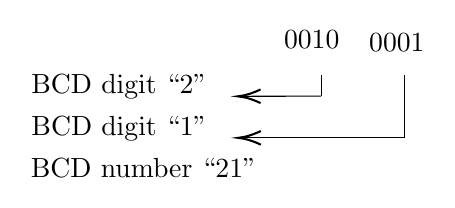
\begin{tikzpicture}[x=0.75pt,y=0.75pt,yscale=-1,xscale=1]
%uncomment if require: \path (0,449); %set diagram left start at 0, and has height of 449

%Straight Lines [id:da19056121715592078] 
\draw    (200.13,320.19) -- (200.13,310.19) ;
%Straight Lines [id:da6977078715888394] 
\draw    (240.13,340.31) -- (240.13,310.06) ;
%Straight Lines [id:da8005164925325152] 
\draw    (200.13,320.19) -- (162,320.31) ;
\draw [shift={(160,320.31)}, rotate = 359.82] [color={rgb, 255:red, 0; green, 0; blue, 0 }  ][line width=0.75]    (10.93,-3.29) .. controls (6.95,-1.4) and (3.31,-0.3) .. (0,0) .. controls (3.31,0.3) and (6.95,1.4) .. (10.93,3.29)   ;
%Straight Lines [id:da5577473383391351] 
\draw    (240.13,340.31) -- (162.13,340.31) ;
\draw [shift={(160.13,340.31)}, rotate = 360] [color={rgb, 255:red, 0; green, 0; blue, 0 }  ][line width=0.75]    (10.93,-3.29) .. controls (6.95,-1.4) and (3.31,-0.3) .. (0,0) .. controls (3.31,0.3) and (6.95,1.4) .. (10.93,3.29)   ;

% Text Node
\draw (59.23,308.5) node [anchor=north west][inner sep=0.75pt]   [align=left] {BCD digit “2”};
% Text Node
\draw (59.27,328.85) node [anchor=north west][inner sep=0.75pt]   [align=left] {BCD digit “1”};
% Text Node
\draw (59,348.96) node [anchor=north west][inner sep=0.75pt]   [align=left] {BCD number “21”};
% Text Node
\draw (181,287.5) node [anchor=north west][inner sep=0.75pt]   [align=left] {0010};
% Text Node
\draw (222,289) node [anchor=north west][inner sep=0.75pt]   [align=left] {0001};


\end{tikzpicture}\\

\noindent\textbf{Exercise 1.16:} \textit{What is the BCD representation for "29"? "91"?}\\

\noindent\textbf{Exercise 1.17:} \textit{Is "10100000" a valid BCD representation? Why?}\\

As many bytes as necessary will be used to represent all BCD digits. Typically, one or more nibbles will be used at the beginning of the representation to indicate the total number of nibbles, i.e., the total number of BCD digits used. Another nibble or byte will be used to denote the position of the decimal point. However, conventions may vary.\\

\noindent{Here is an example of a representation for multibyte BCD integers:}

\tikzset{every picture/.style={line width=0.75pt}} %set default line width to 0.75pt        

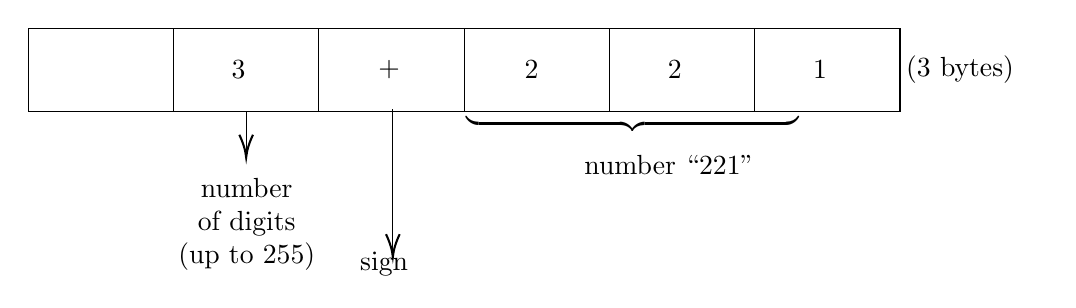
\begin{tikzpicture}[x=0.75pt,y=0.75pt,yscale=-1,xscale=1]
%uncomment if require: \path (0,300); %set diagram left start at 0, and has height of 300

%Shape: Rectangle [id:dp20676377302365134] 
\draw   (50,78) -- (120,78) -- (120,118) -- (50,118) -- cycle ;
%Shape: Rectangle [id:dp21258261570632841] 
\draw   (120,78) -- (190,78) -- (190,118) -- (120,118) -- cycle ;
%Shape: Rectangle [id:dp5882004486829773] 
\draw   (190,78) -- (260,78) -- (260,118) -- (190,118) -- cycle ;
%Shape: Rectangle [id:dp9178100564768983] 
\draw   (260,78) -- (330,78) -- (330,118) -- (260,118) -- cycle ;
%Shape: Rectangle [id:dp2921925051351182] 
\draw   (330,78) -- (400,78) -- (400,118) -- (330,118) -- cycle ;
%Shape: Rectangle [id:dp6058860553033114] 
\draw   (400,78) -- (470,78) -- (470,118) -- (400,118) -- cycle ;
%Straight Lines [id:da7678219758165559] 
\draw    (155,118.25) -- (155,138.25) ;
\draw [shift={(155,140.25)}, rotate = 270] [color={rgb, 255:red, 0; green, 0; blue, 0 }  ][line width=0.75]    (10.93,-3.29) .. controls (6.95,-1.4) and (3.31,-0.3) .. (0,0) .. controls (3.31,0.3) and (6.95,1.4) .. (10.93,3.29)   ;
%Straight Lines [id:da10477434111639439] 
\draw    (225.67,117) -- (225.67,186.17) ;
\draw [shift={(225.67,188.17)}, rotate = 270] [color={rgb, 255:red, 0; green, 0; blue, 0 }  ][line width=0.75]    (10.93,-3.29) .. controls (6.95,-1.4) and (3.31,-0.3) .. (0,0) .. controls (3.31,0.3) and (6.95,1.4) .. (10.93,3.29)   ;

% Text Node
\draw (155,98) node   [align=left] {\begin{minipage}[lt]{10.54pt}\setlength\topsep{0pt}
3
\end{minipage}};
% Text Node
\draw (225,98) node   [align=left] {\begin{minipage}[lt]{9.52pt}\setlength\topsep{0pt}
+
\end{minipage}};
% Text Node
\draw (295,98) node   [align=left] {\begin{minipage}[lt]{8.84pt}\setlength\topsep{0pt}
2
\end{minipage}};
% Text Node
\draw (365,98) node   [align=left] {\begin{minipage}[lt]{10.2pt}\setlength\topsep{0pt}
2
\end{minipage}};
% Text Node
\draw (435,98) node   [align=left] {\begin{minipage}[lt]{10.2pt}\setlength\topsep{0pt}
1
\end{minipage}};
% Text Node
\draw (155.25,172.63) node   [align=left] {\begin{minipage}[lt]{60.74pt}\setlength\topsep{0pt}
\begin{center}
number\\ of digits\\(up to 255)
\end{center}
\end{minipage}};
% Text Node
\draw (208.67,184.33) node [anchor=north west][inner sep=0.75pt]   [align=left] {sign};
% Text Node
\draw (260,118) node [anchor=north west][inner sep=0.75pt]    {$\underbrace{\quad \quad \quad \quad \quad \quad \quad \quad \quad \quad \quad \quad }$};
% Text Node
\draw (366,144) node   [align=left] {\begin{minipage}[lt]{72pt}\setlength\topsep{0pt}
number “221”
\end{minipage}};
% Text Node
\draw (505,98) node   [align=left] {\begin{minipage}[lt]{48pt}\setlength\topsep{0pt}
(3 bytes)
\end{minipage}};
\end{tikzpicture}\\
\noindent{This represents +221}\\
\noindent{(The sign may be represented by 0000 for +, and 0001 for -, for example.)}\\

\noindent\textbf{Exercise 1.18:} \textit{Using the same convention, represent “-23123”. Show it in BCDformat, as above, then in binary.}\\

\noindent\textbf{Exercise 1.19:} \textit{Show the BCD for “222” and “111”, then for the result of 222 $\times$ 111. (Compute the result by hand, then show it in the above representation.)}\\

\noindent{The BCD representation can easily accommodate decimal numbers.}\\
\noindent{For example, +2.21 may be represented by:}\\



\tikzset{every picture/.style={line width=0.75pt}} %set default line width to 0.75pt        

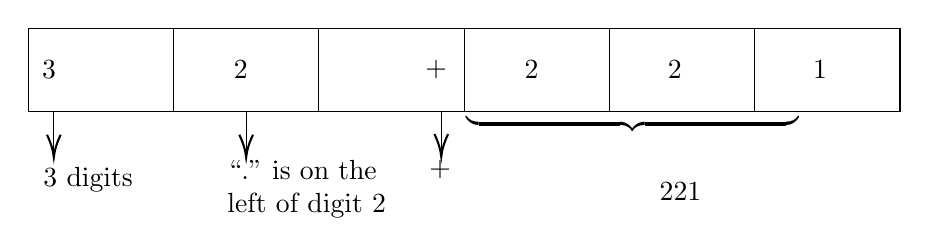
\begin{tikzpicture}[x=0.75pt,y=0.75pt,yscale=-1,xscale=1]
%uncomment if require: \path (0,668); %set diagram left start at 0, and has height of 668

%Shape: Rectangle [id:dp8755983944765307] 
\draw   (58,423) -- (128,423) -- (128,463) -- (58,463) -- cycle ;
%Shape: Rectangle [id:dp3587290468566722] 
\draw   (128,423) -- (198,423) -- (198,463) -- (128,463) -- cycle ;
%Shape: Rectangle [id:dp8445848691125588] 
\draw   (198,423) -- (268,423) -- (268,463) -- (198,463) -- cycle ;
%Shape: Rectangle [id:dp6721518262956601] 
\draw   (268,423) -- (338,423) -- (338,463) -- (268,463) -- cycle ;
%Shape: Rectangle [id:dp8112647214650495] 
\draw   (338,423) -- (408,423) -- (408,463) -- (338,463) -- cycle ;
%Shape: Rectangle [id:dp10540514871316153] 
\draw   (408,423) -- (478,423) -- (478,463) -- (408,463) -- cycle ;
%Straight Lines [id:da8185718082119786] 
\draw    (163,463.25) -- (163,483.25) ;
\draw [shift={(163,485.25)}, rotate = 270] [color={rgb, 255:red, 0; green, 0; blue, 0 }  ][line width=0.75]    (10.93,-3.29) .. controls (6.95,-1.4) and (3.31,-0.3) .. (0,0) .. controls (3.31,0.3) and (6.95,1.4) .. (10.93,3.29)   ;
%Straight Lines [id:da4227711388010926] 
\draw    (257,462.92) -- (257,482.92) ;
\draw [shift={(257,484.92)}, rotate = 270] [color={rgb, 255:red, 0; green, 0; blue, 0 }  ][line width=0.75]    (10.93,-3.29) .. controls (6.95,-1.4) and (3.31,-0.3) .. (0,0) .. controls (3.31,0.3) and (6.95,1.4) .. (10.93,3.29)   ;
%Straight Lines [id:da681868759551965] 
\draw    (70.33,463.25) -- (70.33,483.25) ;
\draw [shift={(70.33,485.25)}, rotate = 270] [color={rgb, 255:red, 0; green, 0; blue, 0 }  ][line width=0.75]    (10.93,-3.29) .. controls (6.95,-1.4) and (3.31,-0.3) .. (0,0) .. controls (3.31,0.3) and (6.95,1.4) .. (10.93,3.29)   ;

% Text Node
\draw (71.67,443) node   [align=left] {\begin{minipage}[lt]{10.54pt}\setlength\topsep{0pt}
3
\end{minipage}};
% Text Node
\draw (255.67,443) node   [align=left] {\begin{minipage}[lt]{9.52pt}\setlength\topsep{0pt}
+
\end{minipage}};
% Text Node
\draw (303,443) node   [align=left] {\begin{minipage}[lt]{8.84pt}\setlength\topsep{0pt}
2
\end{minipage}};
% Text Node
\draw (373,443) node   [align=left] {\begin{minipage}[lt]{10.2pt}\setlength\topsep{0pt}
2
\end{minipage}};
% Text Node
\draw (443,443) node   [align=left] {\begin{minipage}[lt]{10.2pt}\setlength\topsep{0pt}
1
\end{minipage}};
% Text Node
\draw (268,463) node [anchor=north west][inner sep=0.75pt]    {$\underbrace{\quad \quad \quad \quad \quad \quad \quad \quad \quad \quad \quad \ \ \ }$};
% Text Node
\draw (163,443) node   [align=left] {\begin{minipage}[lt]{8.84pt}\setlength\topsep{0pt}
2
\end{minipage}};
% Text Node
\draw (361,496) node [anchor=north west][inner sep=0.75pt]   [align=left] {221};
% Text Node
\draw (64.07,488.52) node [anchor=north west][inner sep=0.75pt]   [align=left] {3 digits};
% Text Node
\draw (152.74,485.19) node [anchor=north west][inner sep=0.75pt]   [align=left] {“.” is on the\\left of digit 2};
% Text Node
\draw (250,485.58) node [anchor=north west][inner sep=0.75pt]   [align=left] {+};


\end{tikzpicture}\\

The advantage of BCD is that it yields absolutely correct results. Its disadvantage is that it uses a large amount of memory and results in slow arithmetic operations. This is acceptable only in an accounting environment and is normally not used in other cases.

\noindent\textbf{Exercise 1.20:} \textit{How many bits are required to encode '9999" in BCD? And in Two's complement?}\\

We have now solved the problems associated with the representation of integers, signed integers and even large integers. We have even already presented one possible method of representing decimal numbers, with BCD representation. Let us now examine the problem of representing decimal numbers in a fixed length for mat.\\

\noindent\textit{Floating-Point Representation}\\

The basic principle is that decimal numbers must be represented with a fixed format. In order not to waste bits, the representation will \textit{normalize} all the numbers.

For example, “0.000123” wastes three zeros on the left of the number, which have no meaning except to indicate the position of the decimal point. Normalizing this number results in .123 $\times$ 103. “.123” is called a \textit{normalized mantissa}, “-3” is called the \textit{exponent}. We have normalized this number by eliminating all the meaning less zeros on the left of it and adjusting the exponent.\\

\noindent{Let us consider another example:}\\

\noindent{22.1 is normalized as $.221 \times 10^2$}\\
\noindent{or $M \times 10^E$ where M is the mantissa, and E is the exponent.}\\

It can be readily seen that a normalized number is characterized by a mantissa less than 1 and greater or equal to .1 in all cases where the number is not zero. In other words, this can be repre sented mathematically by:
\begin{center}
$.1 \leqslant M < 1\ or\ 10^-^1 \leqslant M < 10^0$
\end{center}
Similarly, in the binary representation:
\begin{center}
$2^-^1 \leqslant M<2^0\ (or\ .5\leqslant M<1)$
\end{center}
Where M is the absolute value of the mantissa (disregarding the sign).\\

\noindent{For example:}
\begin{center}
$111.01\ is\ normalized\ as:\ .11101 \times 2^3.$
\end{center}
The mantissa is 11101.\\

\noindent{The exponent is 3.}\\

Now that we have defined the principle of the representation, let us examine the actual format. Atypical floating-point representation appears below.



\tikzset{every picture/.style={line width=0.75pt}} %set default line width to 0.75pt        

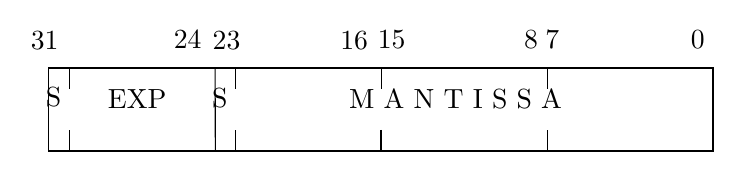
\begin{tikzpicture}[x=0.75pt,y=0.75pt,yscale=-1,xscale=1]
%uncomment if require: \path (0,1248); %set diagram left start at 0, and has height of 1248

%Shape: Rectangle [id:dp6756096304580589] 
\draw   (150.08,630) -- (470.03,630) -- (470.03,670) -- (150.08,670) -- cycle ;
%Straight Lines [id:da4318876624830357] 
\draw    (240.17,660.08) -- (240.17,669.83) ;
%Straight Lines [id:da06530707404660896] 
\draw    (230.14,630.29) -- (230.25,670.42) ;
%Straight Lines [id:da0191016848043416] 
\draw    (160.17,660.08) -- (160.17,670.25) ;
%Straight Lines [id:da10238418718927156] 
\draw    (160.17,629.92) -- (160.17,640.25) ;
%Straight Lines [id:da6367604875756032] 
\draw    (240.17,630.5) -- (240.17,640.25) ;
%Straight Lines [id:da6215778294768212] 
\draw    (310.08,659.83) -- (310.08,669.58) ;
%Straight Lines [id:da049758067482504886] 
\draw    (310.25,630.5) -- (310.25,640.25) ;
%Straight Lines [id:da38179375333111054] 
\draw    (390.17,660.04) -- (390.17,669.79) ;
%Straight Lines [id:da9492802441437873] 
\draw    (390.29,630.37) -- (390.29,640.12) ;

% Text Node
\draw (458.1,610.86) node [anchor=north west][inner sep=0.75pt]   [align=left] {0};
% Text Node
\draw (388,610.86) node [anchor=north west][inner sep=0.75pt]   [align=left] {7};
% Text Node
\draw (377.71,610.9) node [anchor=north west][inner sep=0.75pt]   [align=left] {8};
% Text Node
\draw (307.24,610.95) node [anchor=north west][inner sep=0.75pt]   [align=left] {15};
% Text Node
\draw (289.24,611.48) node [anchor=north west][inner sep=0.75pt]   [align=left] {16};
% Text Node
\draw (227.71,611.38) node [anchor=north west][inner sep=0.75pt]   [align=left] {23};
% Text Node
\draw (208.95,610.9) node [anchor=north west][inner sep=0.75pt]   [align=left] {24};
% Text Node
\draw (140.1,611.38) node [anchor=north west][inner sep=0.75pt]   [align=left] {31};
% Text Node
\draw (147.33,638) node [anchor=north west][inner sep=0.75pt]   [align=left] {S};
% Text Node
\draw (177.24,639.1) node [anchor=north west][inner sep=0.75pt]   [align=left] {EXP};
% Text Node
\draw (227.43,638.81) node [anchor=north west][inner sep=0.75pt]   [align=left] {S};
% Text Node
\draw (293.39,639.37) node [anchor=north west][inner sep=0.75pt]   [align=left] {M A N T I S S A};


\end{tikzpicture}\\
Fig. 1-5: Typical Floating-Point Representation

In the representation used in this example, four bytes are used for a total of 32 bits. The first byte on the left of the illustration is used to represent the exponent. Both the exponent and the mantissa will be represented in two's complement. As a result, the maximum exponent will be -128. “S” in Fig. 1-5 denotes the sign bit.

Three bytes are used to represent the mantissa. Since the first bit in the two's complement representation indicates the sign, this leaves 23 bits for the representation of the magnitude of the mantissa.

\noindent\textbf{Exercise 1.21:} \textit{How many decimal digits can the mantissa repre sent with the 23 bits?}

This is only one example of a floating point representation. It is possible to use only three bytes, or it is possible to use more. The four-byte representation proposed above is just a common one which represents a reasonable compromise in terms of accuracy, magnitude of numbers, storage utilization, and efficiency in arithmetic operation.

We have now explored the problems associated with the representation of numbers and we know how to represent them in in teger form, with a sign, or in decimal form. Let us now examine how to represent alphanumeric data internally.

\noindent\textbf{Representing Alphanumeric Data}

The representation of alphanumeric data, i.e. characters, is com
pletely straightforward: all characters are encoded in an eight-bit
code. Only two codes are in general use in the computer world, the
ASCII Code, and the EBCDIC Code. ASCII stands for *'American
Standard Code for Information Interchange," and is universally
used in the world of microprocessors. EBCDIC is a variation of
ASCII used by IBM, and therefore not used in the microcomputer
world unless one interfaces to an IBM terminal.

Let us briefly examine the ASCII encoding. We must encode 26
letters of the alphabet for both upper and lower case, plus 10
numeric symbols, plus perhaps 20 additional special symbols. This
can be easily accomplished with 7 bits, which allow 128 possible
codes. (See Fig. 1-6.) All characters are therefore encoded in 7 bits.
The eighth bit, when it is used, is the parity bit Parity is a tech
nique for verifying that the contents of a byte have not been ac
cidentally changed. The number of l's in the byte is counted and
the eighth bit is set to one if the count was odd, thus making the
total even. This is called even parity. One can also use odd parity,
i.e. writing the eighth bit (the left-most) so that the total number of
l's in the byte is odd.\\

Example: let us compute the parity bit for "0010011" using even
parity. The number of l's is 3. The parity bit must therefore be a 1
so that the total number of bits is 4, i.e. even. The result is
10010011, where the leading 1 is the parity bit and 0010011 iden
tifies the character.

The table of 7-bit ASCII codes is shown in Fig. 1-6. In practice, it
is used "as is," i.e. without parity, by adding a 0 in the left-most
position, or else with parity, by adding the appropriate extra bit on
the left.

\noindent\textbf{Exercise 1.22:} \textit{Compute the 8-bit representation of the digits "0" through "0", using even parity. (This code will be used in applica tion examples of Chapter 8.)}\\

\noindent\textbf{Exercise 1.23:} \textit{Same for the letters "A " through 44F".}\\

\noindent\textbf{Exercise 1.24:} \textit{Using a non-parity ASCII code (where the left-most bit is "0'7, indicate the binary contents of the 4 bytes below:}
BIT NUMBERS
\
br
\
\
b.
\
♦
b.
\ J
0 0 0 0 0 0 0 0 1 1 1 1 1 1 1 1
b>
\ 0 0 0 0 1 1 1 1 0 0 0 0 1 1 1 1
b,
\ 0 0 1 1 0 0 1 1 0 0 1 J 0 0 1 1
b.
1 0 1 0 1 0 1 0 1 0 1 0 1 0 1 0 1
\HEX1
HEXOS.
0 1 2 3 4 5 6 7 8 9
10
11
12
13
14
15
0
0
0
0
NUL
SOH
STX
ETX
EOT
ENQ
ACK
BEL
BS
HT
LF
VT
FF
CR
SO
SI
0
0
1
1
DLE
DC1
DC2
DC3
DC4
NAK
SYN
ETB
CAN
EAA
SUB
ESC
FS
GS
RS
US
0
1
0
2
SP
1 # $ % & ( ) • + - /
0
3 0 1 2 3 4 5 6 7 8 9 < - > ?
1
0
0
4 m A B C D E F G H 1 J K L M N 0
1
0
1
5 P Q R S T U V W X Y Z [ V ] A _
1
1
0
6 a b c d e f 9 h • i k 1 m n 0
1
1
1
7 P q r s t u V w X y z { 1 }
<^
DEL
Fig. 1-6: ASCII Conversion Table
In specialized situations such as telecommunications, other
codings may be used such as error-correcting codes. However they
are beyond the scope of this book.
32BASIC CONCEPTS
We have examined the usual representations for both program
and data inside the computer. Let us now examine the possible ex
ternal representations.
EXTERNAL REPRESENTATION OF INFORMATION
The external representation refers to the way information is pre
sented to the user, i.e. generally to the programmer. Information
may be presented externally in essentially three formats: binary,
octal or hexdecimal, and symbolic.
1. Binary
It has been seen that information is stored internally in bytes,
which are sequences of eight bits (O's or l's). It is sometimes
desirable to display this internal information directly in its binary
format and this is called binary representation. One simple exam
ple is provided by Light Emitting Diodes (LEDs) which are essen
tially miniature lights, on the front panel of the microcomputer. In
the case of an eight-bit microprocessor, a front panel will typically
be equipped with eight LEDs to display the contents of any inter
nal register. (A register is used to hold eight bits of information
and will be described in Chapter 2). A lighted LED indicates a one.
A zero is indicated by an LED which is not lighted. Such a binary
representation may be used for the fine debugging of a complex
program, especially if it involves input/output, but is naturally
impractical at the human level. This is because in most cases, one
likes to look at information in symbolic form. Thus "9" is much
easier to understand or remember than "1001". More convenient
representations have been devised, which improve the personmachine interface.
2. Octal and Hexadecimal
"Octal" and "hexadecimal" encode respectively three and four
binary bits into a unique symbol. In the octal system, any
combination of three binary bits is represented by a number be
tween 0 and 7.
"Octal" is a format using three bits, where each combination of
three bits is represented by a symbol between 0 and 7:
33PROGRAMMING THE 6502
binary
000
001
010
Oil
100
101
110
111
octal
0 1 2 3 4 5 6 7
Fig. 1-7: Octal Symbols
For example, "00 100
Y T
0 4
or "044" in octal.
Another example: 11
Y 3
or "377" in octal.
100" binary is represented by:
Y 4
111
Y
. 7
111 is:
Y 7
Conversely, the octal "211" represents:
010 001 001
or "10001001" binary.
Octal has traditionally been used on older computers which were
employing various numbers of bits ranging from 8 to perhaps 64.
More recently, with the dominance of eight-bit microprocessors,
the eight-bit format has become the standard, and another more
practical representation is used. This is hexadecimal
In the hex decimal representation, a group of four bits is en
coded as one hexadecimal digit. Hexadecimal digits are
represented by the symbols from 0 to 9, and by the letters A, B, C,
D, E, F. For example, "0000" is represented by "0", "0001" is
represented by "1" and "1111" is represented by the letter "F"
(see Fig. 1-8).
34BASIC CONCEPTS
DECIMAL
0 1 2 3 4 5 6 7 8 9
10
11
12
13
14
15
BINARY
0000
0001
0010
0011
0100
0101
0110
0111
1000
1001
1010
1011
1100
1101
1110
1111
HEX
0 1 2 3 4 5 6 7 8 9 A B C D E F
OCTAL
0 1 2 3 4 5 6 7
10
11
12
13
14
15
16
17
Fig. 1-8: Hexadecimal Codes
35PROGRAMMING THE 6502
Example: 1010 0001 in binary is represented by
A 1 in hexadecimal.
Exercise 1.25: What is the hexadecimal representation of
"10101010?"
Exercise 1.26: Conversely, what is the binary equivalent of "FA "
hexadecimal?
Exercise 1.27: What is the octal of "01000001"?
Hexadecimal offers the advantage of encoding eight bits into on
ly two digits. This is easier to visualize or memorize an# faster to
type into a computer than its binary equivalent. Therefore, on
most new microcomputers, hexadecimal is the preferred method of
representation for groups of bits.
Naturally, whenever the information present in the memory has
a meaning, such as representing text or numbers, hexadecimal is
not convenient for representing the meaning of this information
when it is brought out for use by humans.
Symbolic Representation
Symbolic representation refers to the external representation of
information in actual symbolic form. For example, decimal num
bers are represented as decimal numbers, and not as sequences of
hexadecimal symbols or bits. Similarly, text is represented as
such. Naturally, symbolic representation is most practical to the
user. It is used whenever an appropriate display device is
available, such as a CRT display or a printer. (A CRT display is a
television-type screen used to display text or graphics.) Unfortu
nately, in smaller systems such as one-board microcomputers, it is
uneconomical to provide such displays, and the user is restricted
to hexadecimal communication with the computer.
Summary of External Representations
Symbolic representation of information is the most desirable
since it is the most natural for a human user. However, it requires
an expensive interface in the form of an alphanumeric keyboard,
plus a printer or a CRT display. For this reason, it may not be
36BASIC CONCEPTS
available on the less expensive systems. An alternative type of rep
resentation is then used, and in this case hexadecimal is the domi
nant representation. Only in rare cases relating to fine de-bugging
at the hardware or the software level is the binary representation
used. Binary directly displays the contents of registers of memory
in binary format.
(The utility of a direct binary display on a front panel has always
been the subject of a heated emotional controversy, which will not
be debated here.)
We have seen how to represent information internally and exter
nally. We will now examine the actual microprocessor which will
manipulate this information.
Additional Exercises
Exercise 1,28: What is the advantage of two's complement over other
representations used to represent signed numbers?
Exercise 1.29: How would you represent "1024" in direct binary? Signed
binary? Two's complement?
Exercise 1.30: What is the V-bit? Should the programmer test it after an
addition or subtraction ?
Exercise 1.31: Compute the two's complement of "+16", "+17",
"+18", "-16", "-17", "-18".
Exercise 1.32: Show the hexadecimal representation of the following
text, which has been stored internally in ASCIIformat, with no parity:
= "MESSAGE".


\end{document}